 \documentclass{beamer}

%\usefonttheme{professionalfonts} % using non standard fonts for beamer
%\usefonttheme{serif} % default family is serif
%\usepackage{fontspec}
%\setmainfont{Liberation Serif}

\mode<presentation> {
\usetheme{Malmoe} 
\usecolortheme{beaver} 
}

\usepackage{graphicx} 
\usepackage{booktabs} 
\usepackage{amsmath}
\usepackage{graphicx}
\usepackage[colorinlistoftodos]{todonotes}
\usepackage{hyperref}
\usepackage{multimedia}
\usepackage{media9}
\usepackage{tikz}
\usetikzlibrary{calc,positioning}
\usepackage{xcolor}
\hypersetup{
    colorlinks=true,       
    linkcolor=blue,          
    citecolor=blue,        
    urlcolor=blue           
}
%----------------------------------------------------------------------------------------
%	TITLE PAGE
%----------------------------------------------------------------------------------------

\title[CPS]{\textcolor{black}{{LQR-Trees \cite{p1}}}} 
\subtitle[]{}

\author{George Kontoudis, Shriya Shah}
\institute[VT] 
{
ME5984 Motion Planning Analysis\\
Spring 2017\\
\medskip
\it{Mechanical Engineering Department, Virginia Tech} 
}
\date{\today}

\setbeamertemplate{footline}[text line]{%
  \parbox{\linewidth}{\vspace*{-8pt}\today 
  \hfill\insertshortsubtitle
  \hfill\insertpagenumber}}
\setbeamertemplate{navigation symbols}{}

\begin{document}

\begin{frame}[plain]
\titlepage 
\end{frame}

\begin{frame}
\frametitle{Outline} 
\tableofcontents 
\end{frame}

%----------------------------------------------------------------------------------------
%	PRESENTATION SLIDES
%----------------------------------------------------------------------------------------
%------------------------------------------------
\section{Motivation}
%------------------------------------------------

\begin{frame}
\frametitle{Motivation}
\begin{itemize}
\item  Design robust algorithms for non-linear feedback motion planning \vspace{0.3cm}
\item  Non-linear underactuted systems such as robot manipulator or bipedal walking\vspace{0.3cm}
\item  Computation of planning regions of attraction (funnels) for non-linear underactuated dynamical systems \vspace{0.3cm}
\item Applicable to real robots
\end{itemize}
\end{frame}

%------------------------------------------------
\section{Direct Computation of Lyapunov Functions}
%------------------------------------------------
\subsection{Lyapunov Functions}

\begin{frame}
\frametitle{Definition of Lyapunov Functions}
For a given dynamical system
\begin{equation*}
\dot{x} = f(x), \vspace{.2cm} f(0)=0
\end{equation*} 
a Lyapunov function is $V(x)$, $V\in C$ where
\begin{itemize}
\item $V(x)>0$, positive definite \vspace{0.2cm}
\item $\dot{V}(x)=\frac{dV}{dx} \frac{dx}{dt}<0$, negative definite \vspace{0.2cm}
\end{itemize}
If conditions met in some state space ball $B_r$, then origin is a.s.

\end{frame}

%------------------------------------------------
\begin{frame}
\frametitle{Sequential Composition of Lyapunov Functions}

\begin{columns}[c] 
\column{.56\textwidth}
\begin{itemize}
\item Each funnel acts like a valid Lyapunov function \vspace{0.2cm}
\item A.s. of each Lyapunov falls in the region of attraction of the next lower level \vspace{0.2cm}
\item The lowest function stabilizes in the goal point
\end{itemize}

\column{.54\textwidth} 
\centering
 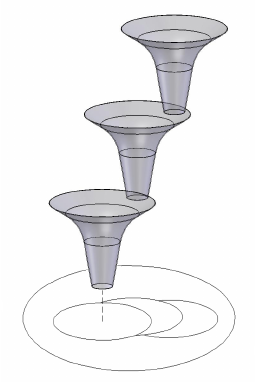
\includegraphics[width=.5\textwidth]{figures/SeqentialLyapunov_Funnels.png}\\
Sequential composition of funnels  \cite{p2}
\end{columns}

\end{frame}


%------------------------------------------------
\subsection{Sum of Squares Validation}
\begin{frame}
\frametitle{Sums of Squares}
We want to check inequalities and validate Lyapunov functions using sums-of-squares (SoS) method \cite{p3}\vspace{.2cm}
\begin{itemize}
\item $x^4+2x^3+3x^2-2x+2 \geq 0, \hspace{.2cm} \forall x \in \mathbb{R}$, by employing SoS
\begin{equation*}
x^4+2x^3+3x^2-2x+2= \begin{bmatrix}
1\\
x\\
x^2
\end{bmatrix}^{\intercal} \begin{bmatrix}
2 & -1 & 0\\
-1 & 3 & 1\\
0 & 1 & 1
\end{bmatrix} \begin{bmatrix}
1\\
x\\
x^2
\end{bmatrix} = X^{\intercal}AX
\end{equation*}
\item Eigenvalues of A are $\lambda_1=3.88$, $\lambda_2=1.65$, $\lambda_1=0.47$, so the inequality stands $\forall x \in \mathbb{R}$
\end{itemize}

\end{frame}

%------------------------------------------------

\begin{frame}
\frametitle{Sums of Squares Properties}
General structure of (SoS) for a 4-$th$ order polynomial is \vspace{.2cm}

\begin{equation*}
fx^4+2ex^3+(d+2c)x^2+2bx+a= \begin{bmatrix}
1\\
x\\
x^2
\end{bmatrix}^{\intercal} \begin{bmatrix}
a & b & c\\
b & d & e\\
c & e & f
\end{bmatrix} \begin{bmatrix}
1\\
x\\
x^2
\end{bmatrix}
\end{equation*}

\begin{itemize}
\item Extend to multivariable polynomials
\item Check non-negativity by searching positive semidefinite matrix
\end{itemize}
\end{frame}

%------------------------------------------------

\begin{frame}
\frametitle{Feedback Synthesis by SoS Optimization}
Given a system $\dot{x} = f(x) + g(x)u$ we want to generate
\begin{itemize}
\item Feedback control law $u=\pi (x)$
\item Lyapunov fcn $V(x)$, s.t.  $V(x)>0$, $\dot{V}(x)=\frac{\partial V}{\partial x}\frac{\partial x}{\partial t}=\frac{\partial V}{\partial x}\dot{x}<0$ 
\end{itemize}\vspace{.5cm}
BUT, this is a difficult problem as the set of $V(x)$, $\pi(x)$ may not be convex sets
\begin{itemize}
\item Rely on LQR synthesis 
\item Design a series of locally-valid controllers 
\item Compose these controllers utilizing feedback motion planning
\end{itemize}
\end{frame}

%------------------------------------------------

\subsection{Complementary - Pontryagin's Principle}

\begin{frame}
\frametitle{The Minimum Principle}
The first order or necessary condition for optimality is called \textit{Maximum (Minimum) Principle} 
\begin{itemize}
\item Given a function we want to minimize $f(x,y,z)$ on a level surface (constraint) $g(x,y,z)$ we get
\begin{equation*}
  \nabla f =\lambda \nabla g
\end{equation*} 
\item To convert a constrained problem to an unconstrained we construct the Hamiltonian function 
\begin{equation*}
  H(x,u,t,\lambda )= L(x,u,t)+ \lambda^{\intercal}f(x,u,t)
\end{equation*}   
\end{itemize}
\end{frame}

%------------------------------------------------
\section{Linear Feedback Design and Verification}
%------------------------------------------------

\subsection{Continuous time LQR}

\begin{frame}
\frametitle{Goal Stabilization}
\begin{itemize}
\item For a given non-linear dynamical system
\begin{equation*}
\dot{x} = f(x,u,t), \hspace{.2cm} x\in \mathbb{R}^n, \hspace{.2cm} u\in \mathbb{R}^m 
\end{equation*} 
\item Set goal state $x_G$, where $f(x_G,u_G)=0$, and $\bar{x}=x-x_G$, $\bar{u}=u-u_G$
\item Linearize around ($x_G, u_G$), $\bar{x}\approx A\bar{x}(t)+B\bar{u}(t)$ 
\item Infinite horizon LQR minimum energy cost-to-go fcn (performance index)
\begin{equation*}
J_{\infty}= \frac{1}{2}\int_0^{\infty} [ \bar{x}^{\intercal}(t)Q\bar{x}(t)+\bar{u}^{\intercal}(t)R\bar{u}(t)]dt,
\end{equation*}
\begin{equation*}
Q=Q^{\intercal}\geq 0, R=R^{\intercal}> 0
\end{equation*}
\end{itemize}
\end{frame}

%------------------------------------------------

\begin{frame}
\frametitle{Hamiltonian System}
Set the Hamiltonian 
\begin{equation*}
H(x,u,t)= L(x,u,t)+\lambda^{\intercal} f(x,u,t)
\end{equation*} 
\begin{itemize}
\item State equation
\begin{equation*}
\dot{x}=\frac{\partial H}{\partial \lambda}
\end{equation*}
\item Costate equation
\begin{equation*}
-\dot{\lambda} = \frac{\partial H}{\partial x}=\frac{\partial f^{\intercal}}{\partial x}\lambda + \frac{\partial L}{\partial x}
\end{equation*}
\item Stationarity condition
\begin{equation*}
0 = \frac{\partial H}{\partial u}=\frac{\partial f^{\intercal}}{\partial u}\lambda + \frac{\partial L}{\partial u}
\end{equation*}
\end{itemize}
\end{frame}

%------------------------------------------------

\begin{frame}
\frametitle{Riccati equation and Optimal Control Law}
\begin{itemize}
\item Infinite horizon LQR problem results the optimal cost
\begin{equation*}
J^{\ast}(\bar{x})=\frac{1}{2}\bar{x}^{\intercal}S\bar{x}
\end{equation*} 
\item $S > 0$, w/ the solution given from ARE
\begin{equation*}
0=Q-SBR^{-1}B^{\intercal}S+SA+A^{\intercal}S
\end{equation*}
\item Optimal feedback closed loop control policy 
\begin{equation*}
\bar{u}^{\ast}=-R^{-1}B^{\intercal}S\bar{x}=-Kx
\end{equation*}
\end{itemize}
\end{frame}


%------------------------------------------------
\subsection{State LQR Verification}

\begin{frame}
\frametitle{Goal State Convergence}
The domain of attraction of the LQR over some sub-level set
\begin{equation*}
B_G(\rho)=\{ x|0\leq V(x) \leq \rho \} 
\end{equation*} 
To guarantee a.s. we require $V(x)$ to be a valid Lyapunov function
\begin{itemize}
\item $V(x)>0, \hspace{.2cm} x\in B_G(\rho)$
\item $\dot{V}(x)<0, \hspace{.2cm} x\in B_G(\rho)$
\end{itemize}
\vspace{.4cm}
Assign $V(x)=J^{\ast}(\bar{x}) = \frac{1}{2}\bar{x}^{\intercal}S\bar{x}$
\begin{itemize}
\item By definition positive definite
\item $\dot{V}(x)=\dot{J}(\bar{x})=\frac{dV}{dx} \frac{dx}{dt} = 2\bar{x}^{\intercal}S\dot{x} = 2\bar{x}^{\intercal}Sf(x_G+\bar{x}, u_G-K\bar{x}) $
\end{itemize}
\end{frame}

%------------------------------------------------

\begin{frame}
\frametitle{Lyapunov Verification Using SoS}
We require 
\begin{equation*}
\dot{J}^{\ast}(\bar{x})<0, \hspace{.4cm} \forall\bar{x} \neq 0 \in B_G(\rho), \hspace{.4cm} \dot{J}^{\ast}(0)=0
\end{equation*} 
\begin{itemize}
\item First, modify the inequality from negative to non-positive 
\begin{equation*}
\dot{J}^{\ast}(\bar{x})\leq -\epsilon ||\bar{x}||_2^2, \hspace{.4cm} \forall \bar{x}\in B_G(\rho),\hspace{.4cm} \epsilon \in \mathbb{R}^+
\end{equation*}
\item Second, include the constraint with Lagrange multiplier $h(\cdot)$
\begin{equation*}
\dot{J}^{\ast}(\bar{x})+ h(\bar{x})(\rho - J^{\ast}(\bar{x}))\leq -\epsilon ||\bar{x}||_2^2
\end{equation*}
\end{itemize}
\end{frame}

%------------------------------------------------

\begin{frame}
\frametitle{Lagrange Mulitplier Searching}
\begin{itemize}
\item If $f^{(cl)}(x,u)=f(x,u_G-K(x-x_g))$, search for $h(\cdot)$ polynomial with sufficient order for $\dot{J}^{\ast}(\bar{x})$, using SoS
\begin{center}
\begin{tabular}{ r l }
find & $h(\bar{x})$ \\
subject to & $\dot{J}^{\ast}(\bar{x})+ h(\bar{x})(\rho - J^{\ast}(\bar{x}))\leq -\epsilon ||\bar{x}||_2^2$\\
 & $h(\bar{x})\geq 0$
\end{tabular}
\end{center}
\item If $f^{(cl)}(x)\approx \hat{f}^{(cl)}(\bar{x})$, where $\hat{f}^{(cl)}(\bar{x})$ is the Taylor expansion (algebraic approximation) and $\hat{\dot{J}}(\bar{x})=2\bar{x}^{\intercal}S\hat{f}^{(cl)}(\bar{x})$
\begin{center}
\begin{tabular}{ r l }
find & $h(\bar{x})$ \\
subject to & $\hat{\dot{J}}(\bar{x})+ h(\bar{x})(\rho - \hat{J}^{\ast}(\bar{x}))\leq -\epsilon ||\bar{x}||_2^2$\\
 & $h(\bar{x})\geq 0$
\end{tabular}
\end{center}
\end{itemize}

\end{frame}

%------------------------------------------------

\begin{frame}
\frametitle{Optimization for $\rho$}
Set a convex optimization problem for the region of attraction 
\begin{center}
\begin{tabular}{ r l }
max & $\rho$ \\
subject to & $\hat{\dot{J}}^{\ast}(\bar{x})+ h(\bar{x})(\rho - \hat{J}^{\ast}(\bar{x}))\leq -\epsilon ||\bar{x}||_2^2$\\
 & $h(\bar{x})\geq 0$\\
 & $\rho>0$
\end{tabular}
\end{center}
\begin{columns}[c] 
\column{.56\textwidth}
\begin{itemize}
\item At each step the Lagrange multiplier searching is performed
\item If the program is feasible $\rho$ increased 
\end{itemize}

\column{.56\textwidth}
\centering
 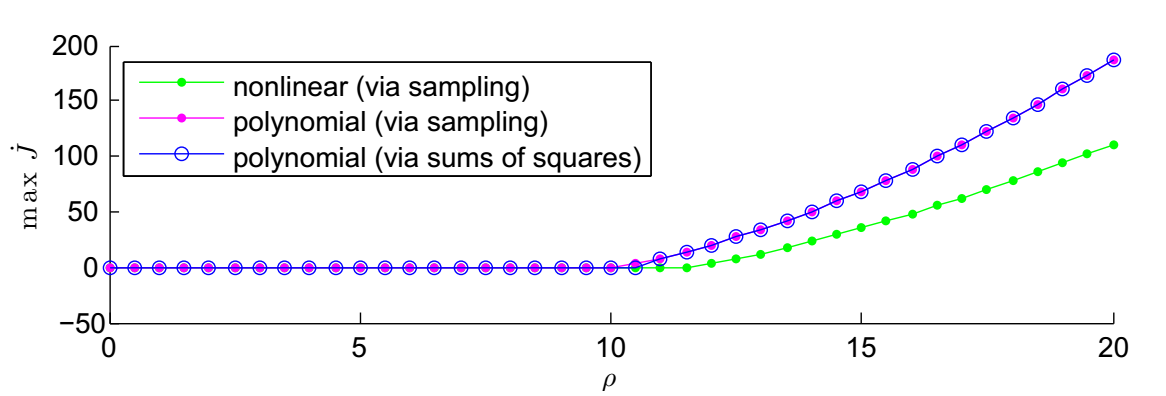
\includegraphics[width=.95\textwidth]{figures/PolynomialVerification.png}\\
Polynomial verification of damped single pendulum  \cite{p1}
\end{columns}

\end{frame}

%------------------------------------------------

\subsection{Trajectory Optimization}
\begin{frame}
\frametitle{Trajectory Optimization}

\end{frame}

%------------------------------------------------
\subsection{Trajectory LQR Verification}

\begin{frame}
\frametitle{Time-Invariant LQR Verification}

\end{frame}

%------------------------------------------------

\section{Conclusions}
\begin{frame}
\frametitle{Conclusions}

\end{frame}

%------------------------------------------------
\section{References}
%------------------------------------------------

\begin{frame}
\frametitle{References}
\footnotesize{
\begin{thebibliography}{99} % Beamer does not support BibTeX so references must be inserted manually as below

%@article{tedrake2010lqr,
%  title={LQR-trees: Feedback motion planning via sums-of-squares verification},
%  author={Tedrake, Russ and Manchester, Ian R and Tobenkin, Mark and Roberts, John W},
%  journal={The International Journal of Robotics Research},
%  volume={29},
%  number={8},
%  pages={1038--1052},
%  year={2010},
%  publisher={SAGE Publications Sage UK: London, England}
%}

\bibitem[Tedrake, 2010]{p1} R. Tedrake, I. Manchester, M. Tobenkin, and J. Roberts
\newblock LQR-trees: Feedback motion planning via sums-of-squares verification
\newblock \emph{International Journal of Robotics Researchs, 1038--1052, SAGE Publications}, 2010.

%@article{burridge1999sequential,
%  title={},
%  author={Burridge, Robert R and Rizzi, Alfred A and Koditschek, Daniel E},
%  journal={The International Journal of Robotics Research},
%  volume={18},
%  number={6},
%  pages={534--555},
%  year={1999},
%  publisher={Sage Publications}
%}

\bibitem[Burridge, 1999]{p2} R. Burridge, A. Rizzi, and D. Koditschek
\newblock Sequential composition of dynamically dexterous robot behaviors
\newblock \emph{International Journal of Robotics Researchs, 534--555, SAGE Publications}, 1999.

%@phdthesis{parrilo2000structured,
%  title={Structured semidefinite programs and semialgebraic geometry methods in robustness and optimization},
%  author={Parrilo, Pablo A},
%  year={2000},
%  school={Citeseer}
%}

\bibitem[Parrilo, 2000]{p3} P.Parrilo
\newblock Structured semidefinite programs and semialgebraic geometry methods in robustness and optimization
\newblock \emph{Ph.D. Theis, MIT}, 2000.


\end{thebibliography}
}
\end{frame}

%------------------------------------------------
\section{}
\begin{frame}
\begin{center}
\Huge {Thank You!}
\end{center}
\end{frame}

%----------------------------------------------------------------------------------------

\end{document} 